%!TEX root = ../thesis.tex
% NIR-information

\chapter{NIR information}

\label{cha:nir_content}

\section{Overview}

The pursuit of detecting exoplanets, especially ``habitable'' and ``Earth-like'' planets, requires state-of-the-art instrumentation with high precision. One of the key detection methods, the Radial Velocity (RV) method, measures the wobble induced on the Star by the planet as they orbit their common barycenter \reference{rv method}.  {\red{} add Some stuff about mass and period from pedros paper}



A increase in the number of \nir{} spectrographs is increasing to focus on cooler M-dwarfs stars which have a easier* chance of detecting Earth-like planets in the habitable zone. \change{Check mission statements for these}{SPIRou, NIRPS} and CARMENES. Also CRIRES+...
This work continues the assessment of RV precision levels possible in this domain.
\todo{For example from Figueira 2016 see figure) A more precise measurement can be achieved from X band then the Y band... or in order XYZ of precision}

\missingfigure{An example from Figueira et al. 2016}



This work is not directly related to detecting exoplanet atmospheres themselves but investigates the theoretical and observed RV precision of M-dwarf spectra in the NIR. This has previously helped the aid the direction of instrument design by identifying the wavelength regions with the best RV precision \citep{figueira_radial_2016} but can also help in the planning of observations, by understanding how the precision changes with spectral type and observed SNR. This can help in detecting the presence of ``habitable Earth-like'' planets around M-dwarfs which will likely have their atmospheres evenutally probed.


\section{Radial velocity precision}
The first detections of planets with the RV technique \textbf{Queloz 2995} discovered the mass and close in hot-Jupiter planets. These are the easiest to detect with the highest RV amplitude.

Over the years the community has push the limits of this technique to smaller and smaller planetary masses. An example is shown in Fig.~\ref{fig:year_mass}.
\begin{figure}

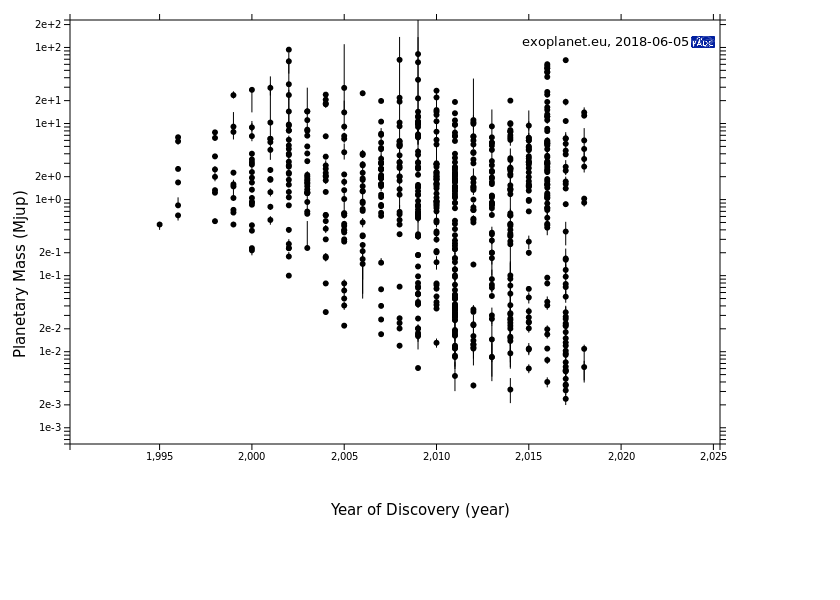
\includegraphics[width=0.8\linewidth]{figures/year_planet_mass.png}
\caption{Mass of discovered planets verse year. From Exoplanet.eu}
\label{fig:year_mass}
\end{figure}


RV amplitude scales with mass of the star $M_\star^{-2/3}$ and with the planetary orbital period $P_\textrm{orb}^{-2/3}$.

The detection of an Earth-mass planet inside the habitable zone around a solar-type star, the RV amplitude is 10 cm/s. If that a planet with the same characteristics is instead orbiting a M/ -dwarf, the RV amplitude is larger than 1 m/s. This is due to two factors, the smaller mass of the host star, and the closer habitable zone, due to a lower luminosity output of the host)

\citet{artigau_optical_2018} recently compared archival spectra of Barnard's Star, an M-dwarf, and found that state-of-the-art atmosphere models over-predict the $Y$ and $J$-band RV content by more than a factor of $\sim$$2$, while under-predicting the $H$ and $K$-band content by half.
{\red{} in this work we find similar?}

We are currently aiming to extend this work over the whole M-dwarf range, from M0-M9.


History of Precision calculations:
Connes 1985 -
Bouchy et al. 2001  - photon noise limit on rv measurements.
Figueria et al. 2016 - focus on m-dwarfs parameter range to specify new instrumentation windows to focus.
Reiners 2017 -  Carmenes sample. some precision
pedros school section other precision source r\^1.5


\subsection{Fundamental photon noise limitation}

A optimum technique to calculate the radial velocity precision of a spectrum using the full spectral information is proposed by~\citet{Connes1985}. Here we provide the radial velocity precision derivation following~\citet{Connes1985, bouchy_fundamental_2001, figueira_radial_2016}. A majority of this derivation comes from~\citet{bouchy_fundamental_2001} with some extra notes added to improve the clarity.

For each spectrum there is assigned a quality factor, Q, to compute the fundamental uncertainty on the radial velocity measurements due to noise. {\red{} i am not sure what i am trying to say in this sentence}\unfinished{Change picture spectral range to capital lambda $\Lambda$}

\begin{figure}
    \centering
    %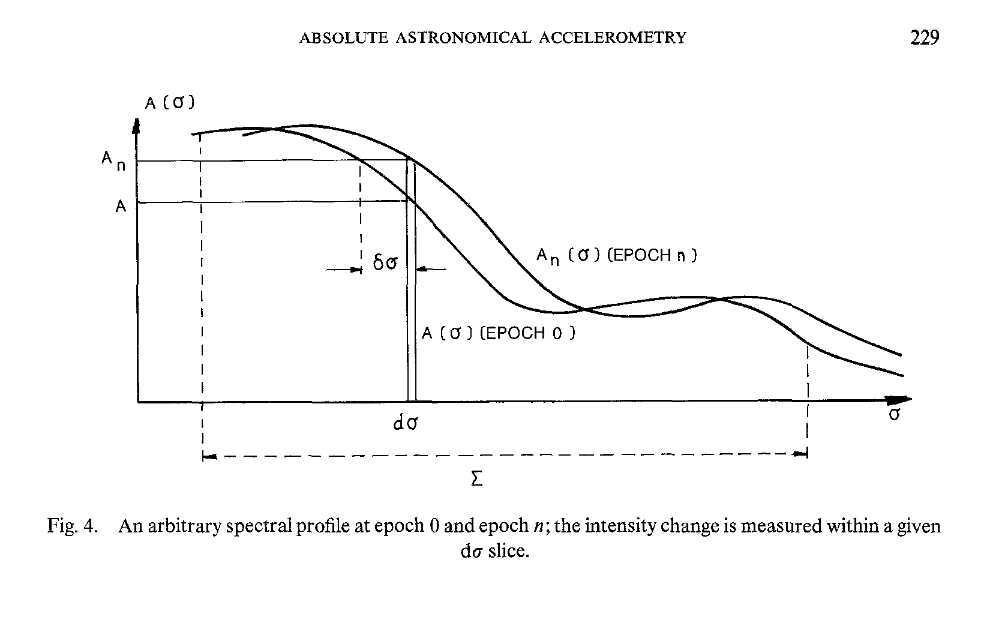
\includegraphics[width=0.7\linewidth]{figures/spectrum_example_a}
   % 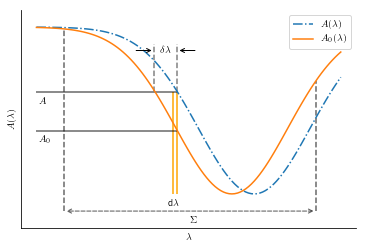
\includegraphics[width=0.7\linewidth]{figures/precision_derivation.pdf}
    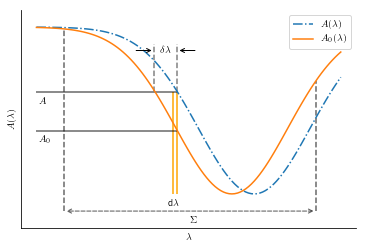
\includegraphics[width=0.7\linewidth]{figures/precision_derivation.png}
    \caption{Arbitrary spectral line with a shift $\delta \lambda$, inspired by~\citet{Connes1985}.  \(\Lambda\) is the wavelength range considered.}
    \label{fig:precisionderivation}
\end{figure}

The Doppler shift of a spectrum is given by:
\begin{equation}
\frac{\delta V}{c} = \frac{\delta \lambda}{\lambda}.
\label{eq:dopplershift}
\end{equation}
Here $c$ is the speed of light in a vacuum, and $\delta \lambda$ is the observed shift in wavelength $\lambda$ caused by the velocity $\delta V$

Using basic calculus \(\delta y = \frac{\partial y}{\partial x} \delta x,  \nonumber\) and for a Doppler shift that is small compared to the line-width\footnote{Although~\citet{Connes1985} show that this approximation in Eq.\,\ref{eq:intensitychange} is adequate under all circumstances}, the observable intensity change at a given pixel can be expressed by:

\begin{equation}
\delta A(i) = A(i) - A_0(i) \simeq \frac{\partial A_0(i)}{\partial \lambda} \delta \lambda
\label{eq:intensitychange}
\end{equation}

Rearranging Eq.~\ref{eq:intensitychange} for \(\delta \lambda\) and putting it into Eq.~\ref{eq:dopplershift}, the Doppler shift of then becomes:
\begin{equation}
    \frac{\delta V(i)}{c} = \frac{A(i) - A_0(i) }{\lambda(i) (\partial A_0(i)/\partial \lambda(i))} \label{eq:delta_v_i}
\end{equation}

This equation shows that the changes in velocity is measured through a change in intensity in the recorded spectrum, \(A(i)-A_0(i)\), and inversely proportional to the slope of the spectrum, \(\partial A_0(i)/\partial \lambda(i))\).
This equation provides a measurement of the radial velocity shift for each pixel (i) in the spectrum. The whole available spectral range, $\Sigma$, should be used to increase the sensitivity of the measurement and decrease the noise. This is achieved by summing the contribution of all pixels using an optimal weight W(i).

\begin{equation}
\frac{\delta V}{c} = \frac{\Sigma{ \frac{\delta V(i)}{c}W(i)}}{\Sigma {W(i)}}
\end{equation}

Statistically, the optimal weights are proportional to the inverse square of the individual dispersion,


\begin{equation}
W(i) = \frac{1}{\left(\frac{\delta V_{RMS}(i)}{c}\right)^2},  \label{eq:weights}
\end{equation}
where $X_{RMS}$ is the dispersion on the quantity $X$.


The individual dispersion of the velocity change measure $\delta V_{RMS}(i)$ is the dispersion of radial velocity resulting from several measurements of the reference spectrum all with the same Doppler shift (e.g. zero). Equation.\,\ref{eq:delta_v_i} thus becomes:
\begin{equation}
    \frac{\delta V(i)}{c} = \frac{{[A(i) - A_0(i)]}_{RMS} }{\lambda(i) (\partial A_0(i)/\partial \lambda(i))} \label{eq:delta_v_i_rms}
\end{equation}
The noise of the spectrum A is the quadratic sum of the photon noise \(\sqrt{A}\) and the detector noise \(\sigma_D\). The spectrum \(A_0\) is considered noise free.

\begin{equation}
[A(i)-A_0(i)]_{RMS} = [A(i)]_{RMS} = \sqrt{\sqrt{A(i)}^2 + \sigma^2_{D}} \label{eq:noise}
\end{equation}
We can set \(A = A_0\) if we consider the Doppler shift is small and that \(A\) and \(A_0\) have the same intensity level. Using Eq.\,\ref{eq:weights},\,\ref{eq:delta_v_i} and\,\ref{eq:noise}	the optimum weights then become solely dependent on the reference spectrum.



\begin{equation}
W(i) =   \frac{\lambda^2(i)  (\partial A_0(i)/\partial \lambda(i))^{2}}{A(i) + {\sigma}^{2}_{D}} \label{eq:optimal_weight}
\end{equation}
This weighting function can be modified to mask out and eliminate unwanted lines in the spectrum. For instance in the removal of telluric absorption lines in observed spectra. This is achieved to setting the particular pixel weights to zero.

With the optimal weights set the velocity change measured from the full spectral range \(\Lambda\), \unfinished{Change picture spectral range} is given by:


\begin{eqnarray}
    \frac{\delta V(i)}{c} &= \frac{
    	\Sigma{
        	\frac{
            	A(i) - A_0(i)}{
                \lambda(i) \left(\partial A_0(i)/\partial \lambda(i)\right)} W(i)}}{
             \Sigma {W(i)}} \\
    &= \frac{
    	\Sigma  {
        	(\frac
            	{A(i) - A_0(i)}
                {\lambda(i) (\partial A_0(i)/\partial \lambda(i))}) \frac
                	{\lambda^2(i)  (\partial A_0(i)/\partial \lambda(i))^{2}}
                    {A(i) + {\sigma}^{2}_{D}}
                 }
         }
    {\frac
    	{\lambda^2(i)  (\partial A_0(i)/\partial \lambda(i))^{2}}{A(i) + {\sigma}^{2}_{D}}
        } \\
    &=
    \label{eq:delta_v_eqarray}
\end{eqnarray}\unfinished {Finish this equation (9 of bouchy 2001)}
\unfinished{Try the symbolic package from PC}

The important quantity for RV measurements is not only the velocity value itself but the dispersion on the measured velocity or the precision, \(\delta V_{RMS}\). From equation \ref{eq:weights} the dispersion is given by :


\begin{equation}
    \frac{\delta V_{RMS}}{c} = \frac{1}{\Sigma {\,W(i)}} = \frac{1}{Q \Sigma {\,A_0(i)}}
\end{equation}
With this the velocity precision is inversely proportional to the sum of the optimal pixel weights.

A spectral quality factor, Q, is defined as for the pure photon noise case, as in~\cite{Connes1985, connes_demonstration_1996}.

\begin{equation}
Q = \frac{\sqrt{\Sigma{\,W(i)}}}{\sqrt{\Sigma{\,A_0(i)}}}.
\end{equation}
This factor is flux independent and is purely a function of the spectral profile within the spectral range considered. It is is a measure of the line richness. For example a spectra with many sharp lines will have a high Q. This quality factor is valid for the pure photon noise case only.

With this quality factor the uncertainty in the velocity change can be rearranged in terms of the spectral quality;

\begin{equation}
    \delta V_{RMS} = \frac{c}{Q \sqrt{\Sigma {\,A_0(i)}}} = \frac{c}{Q \sqrt{{N}_{{e}^{-}}}},
\end{equation}

where \(\Sigma A_0(i) = {N}_{{e}^{-}}\) is considered to be the total number of photo electrons \({N}_{{e}^{-}}\) counted in the whole spectral range considered.
From the spectral quality factor and the number of photons collect the fundamental velocity precision can be determined.

The spectral quality depends on the spectral profile of the target as well as the instrumental resolution of the spectrograph (which induces line broadening). The number of photoelectrons counted  \(N_{e^{-}}\) depends on the stellar magnitude, detector efficiency and integration time. It can be estimated using
 \begin{equation}
 N_{e^{-}} = P_{avg} * S_{tel} * T_{exp} * \alpha* \Lambda,
 \end{equation}

where \(P_{avg}\) is the average monochromatic stellar brightness
across the wavelength range \(\Lambda\) in

\si{\photons\per\second\per\centi\metre\squared\per\centi\metre},

\(S_{tel}\) is the telescope collecting area in \si{\centi\metre\squared},

\(T_{exp}\) is the integration time in \si{\second},

and \(\alpha\) the overall efficiency (including atmosphere, telescope, spectrograph and detector).

 This can be used to determine the RV precision for a given instrument, and be useful in exposure time calculators for planing observations.

In the case of several \(\delta V\) measurements computed for \(k\) spectral slices (or spectral orders) then the error on the average \(\delta V\) is given by the error on a weighted average:
\begin{equation}
\overline{\delta {V}_{RMS}} = \frac{1}{\sqrt{\Sigma_k{(\frac{1}{\delta V_{RMS}(k)})^2}}}
\end{equation}


We follow~\cite{figueira_radial_2016} by exclusively considering a high signal-to-noise regime in which $A(i) + D^2 \sim A(i)$ can be approximated.


\footnote{ pure detector noise the fluctuation are independent of the spectrum \(A\) and the quality factor for pure detector noise is \(Q_D = \frac{\Sigma{\lambda^2 {(\partial A_0(i)/\partial \lambda(i))}^{2}}}{\Sigma{\, A_0(i)}}\) as derived by~\cite{Connes1985}. }

The in the photon noise limited case we assume that all measurements have same RV then the the the object has not
\citet{Connes1985} show that the optimal weights for photon limited noise is given by.....

There is also a optimal weight for detector noise but we are always assume we are in high SNR case and are photon noise limited.


This technique has been tested and demonstrated on observations by~\citet{connes_demonstration_1996} and been used to determine predict the accuracy or performance limits of spectrograph instrumentation~\citet{Connes1985,bouchy_fundamental_2001} and can influence the design (or use) of spectrographs
 (e.g. SPIROU~\citep{artigau_spirou_2014,figueira_radial_2016})
\unfinished{Does spectrograph pipelines such as HARPS use these equations to measure estimate/precision?}


Considering that \(\Sigma{A_0(i)} = N_{e^-} \) is the total number of photoelectrons counted over the whole spectral range then the uncertainty in the velocity change is finally given by:

\begin{equation}
\frac{\delta V_{RMS}}{c} = \frac{c}{Q \sqrt{N_{e^-}}} \approx \frac{c}{Q (S/N)},
\end{equation}

where the \(SNR=\sqrt{N_{e^-}} \)for large N. \unfinished{It is convenient to use this version when comparing observed spectra with different S/N.?}




\subsection {Signal to noise scaling}
Take 1 sampling width at center of band - > scale to specific snr require.
provide the scaling default spectral SNR.
new precision = old precision * old snr / new snr

We should provide the resolution element 3 pixel snr value from the code...


\subsection{Prepare phoenix aces models}:
\# see~\citet{figueira_radial_2016}

Convert SED to counts.


Scale to 100 snr per resolution element in J band.

Convolutions


Since the synthetic models do not have a consistent wavelength grid, the discretization of the convolution kernel onto the changing wavelength grid causes each pixel to be multiplied by a slightly different kernel area. We therefore divide the result by a convolution of a spectrum of ones with the same wavelength resolution.

Differences to Figueria et al.

%-----------------------------------
%	SUBSECTION 2
%-----------------------------------

Preparation of Carmenes spectra.


\missingfigure{Example of CARMENES spectra before and after correction}

\subsection{Bands}
The bands are selected based on the strong water absorption. This can be seen the Carmenes spectra in Figure~\ref{}\todo{Add figure here}. The wavelength ranges used in this work \citet{figueira_radial_2016} and used in this work are given in Table~\ref{tab:band_ranges}.
\begin{table}
    \centering
    \caption{The wavelength ranges of the \nir{} spectral bands.}
    \begin{tabular}{cc}
        \toprule
        Band & Range (\um{})\\
        \midrule
        Z & 0.83 -- 0.93\\
        Y & 1.00 -- 1.10\\
        J & 1.17 -- 1.33\\
        H & 1.50 -- 1.75\\
        K & 2.07 -- 2.35\\
        \bottomrule
    \end{tabular}
    \label{tab:band_ranges}
\end{table}



\subsection{Comparing models to Carmenes.}
Already somewhat done in Reiners. (use all spectra). They measured the precision obtained in the spectra.

Band by band like Figueria 2016?
Certain\% steps like Bouchy or Artigau


Can do Barnard's star in CARMENES. compared to models in Artigau.

\DTLsetseparator{,}
\DTLloadrawdb{targets}{data/carmenes_selection.csv}%

\begin{table*}[b]
    \centering
    \caption{CARMENES library target selection spanning the M-Dwarf spectral range.}
    \begin{tabular}{l l l r c c c c}%
        \toprule
        Karmn & Name & SpT &  $\textrm{SNR}_{\textrm{NIR}}$  & Temp (K) & logg & [Fe/H] & v$\sin{i}$ (km/s)\\
        \midrule
        \DTLforeach*{targets}{\id=Karmn,\name=Name,\sptype=SpT,\snr=NIR-SNR,\teff=Teff, \logg=logg,\metal=FeH, \rot=ROT-Vsini}{
            \DTLiffirstrow{}{\\}\id & \name &\sptype & \snr & \teff & \logg & \metal & \rot
        }
        \\
        \bottomrule
    \end{tabular}
    \label{tab:targets}
\end{table*}

%!TEX root = ../thesis.tex

\begin{table}[h]
    \caption{csv2tex table}
    \begin{tabular}{lllrrrrr}
        \toprule
        Karmn &            Name &   SpT &  NIR-SNR &    Teff &  logg &   FeH &  ROT-Vsini \\
        \midrule
        J20533+621 &      BD+61 2068 &  M0.5 &      257 &  3772.0 &     - & -0.01 &       2.66 \\
        J04290+219 &       BD+21 652 &  M0.5 &      212 &  4037.0 &  3.99 & -0.21 &       1.11 \\
        J07274+052 &   Luyten's Star &  M3.5 &      254 &  3467.0 &     - & -0.11 &          - \\
        J17578+046 &  Barnard's Star &  M3.5 &      236 &  3247.0 &     - & -0.32 &          - \\
        J11055+435 &          WX UMa &  M5.5 &      140 &  3304.0 &     - &     - &          - \\
        J10564+070 &          CN Leo &  M6.0 &      133 &  2960.0 &     - &     - &          - \\
        J18356+329 &  LSR J1835+3259 &  M8.5 &       50 &  2578.0 &     - & -0.40 &      37.60 \\
        J04198+425 &  LSR J0419+4233 &  M8.5 &       42 &       - &     - &  0.22 &          - \\
    \bottomrule
    \end{tabular}\label{tab:carmenes_selection}
\end{table}

%\begin{table}
\label{}
\caption{csv2tex table transposed}
\begin{tabular}{lllllllll}
\toprule
{} &           0 &           1 &              2 &               3 &           4 &           5 &               6 &               7 \\
\midrule
Karmn     &  J20533+621 &  J04290+219 &     J07274+052 &      J17578+046 &  J11055+435 &  J10564+070 &      J18356+329 &      J04198+425 \\
Name      &  BD+61 2068 &   BD+21 652 &  Luyten's Star &  Barnard's Star &      WX UMa &      CN Leo &  LSR J1835+3259 &  LSR J0419+4233 \\
SpT       &        M0.5 &        M0.5 &           M3.5 &            M3.5 &        M5.5 &        M6.0 &            M8.5 &            M8.5 \\
NIR-SNR   &         257 &         212 &            254 &             236 &         140 &         133 &              50 &              42 \\
Teff      &        3772 &        4037 &           3467 &            3247 &        3304 &        2960 &            2578 &               - \\
logg      &           - &        3.99 &              - &               - &           - &           - &               - &               - \\
FeH       &       -0.01 &       -0.21 &          -0.11 &           -0.32 &           - &           - &            -0.4 &            0.22 \\
ROT-Vsini &        2.66 &        1.11 &              - &               - &           - &           - &            37.6 &               - \\
\bottomrule
\end{tabular}
\end{table}


\section{Metallicity logg effects}
We explore the effect of metallicity and logg on the spectral quality of spectra in the PHOENIX-ACES library by extending the quality factor and precisions computation to [Fe/H] -1--1 and logg 4.0--5.5. In figure \ref{fig:deviations} show the variation of quality factor with broadening of R=100000 and vsini=1.0 km/s across the M-dwarf spectral types and the \nir{} bands. We observed multiple different effects present.


The Z band has a large separation in spectral quality due to spectral type, this is because the continuum the Z band is severely eroded in the spectra of late M's as they cool. Each spectral type also behaves very differently to a change in [Fe/H] and logg. For M0 and M3 there is an increase with [Fe/H] below solar metallicity, above solar metallicity the slopes of the lines dramatically increase, especially for M3. For M6 and M9 there is a step slope with [Fe/H] below solar metallicity, which flattens off at solar metallicity, and even decreases for the M9 spectra above solar metallicity.
As logg increases in the Z band there is a decrease in quality. There is a consistently large separation between early and late M's that. The quality for M6 is very shallow, while for M9 the quality is nearly flat for logg = 4.0 and 4.5 but then decreases sharply at higher logg.

Y band -\\

J band - \\

For the H and K band there is fairly consistent linear trend for all spectral types, with the quality factor increasing with an increase in [Fe/H] and decreasing with an increase in logg. There is also only a relatively small variation in quality factor due to the spectral type.



\begin{figure}
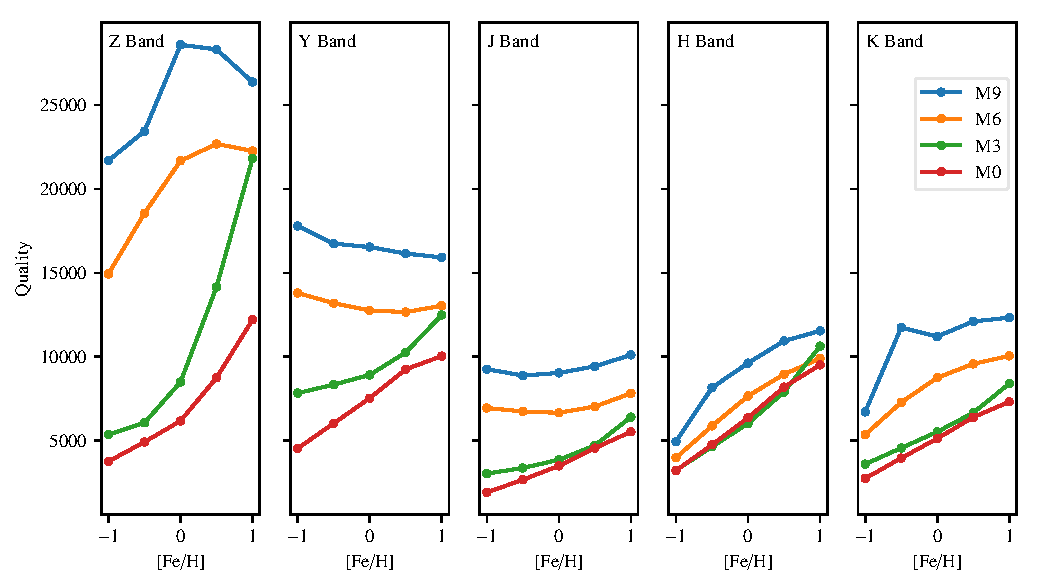
\includegraphics[width=0.99\linewidth]{figures/information-content/metalicity_effect.pdf}\\
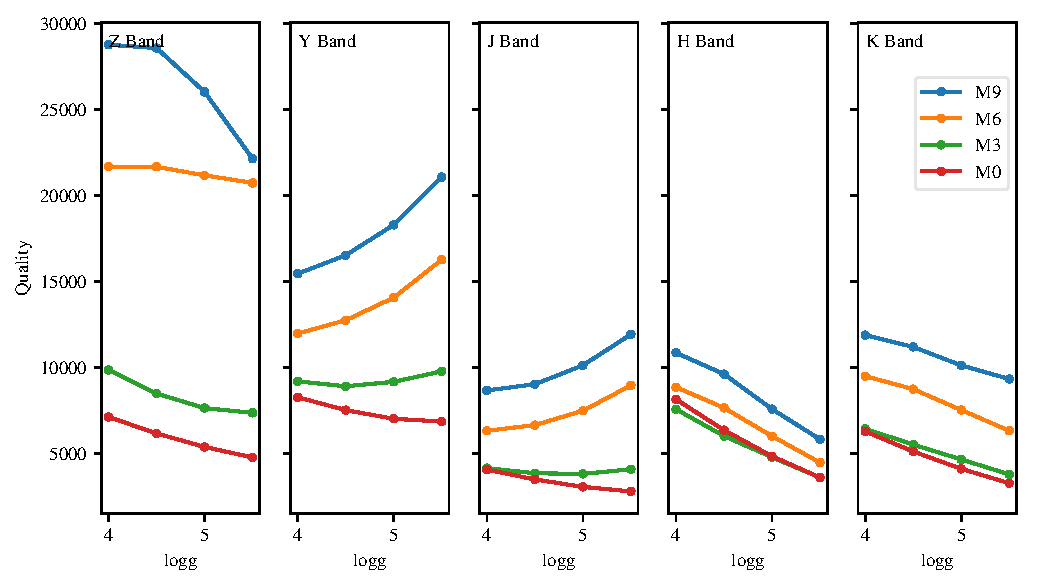
\includegraphics[width=0.99\linewidth]{figures/information-content/logg_effect.pdf}
\caption{Quality factor changes across spectral type and bands for variations in [Fe/H] and logg. Broadening values are R=100000 and vsini = 1.0 km/s. Top: Quality factor variation of [Fe/H] between -1.0 to 1.0 at a fixed logg=4.5. Bottom: Quality factor variation of logg between 4 and 5.5 with fixed [Fe/H]=0.0. Note a higher quality factor corresponds to an increased RV precision.}
\label{fig:deviations}
\end{figure}

%----------------------------------------------------------------------------------------
%	SECTION 2
%----------------------------------------------------------------------------------------

\section{Main Section 2}



\section{Code improvements}
Care needs to be taken to optimize the code. The original code used in Figueira 2016 was very slow, taking around 2 hours per simulation, this lead to weeks of processing time to compute the precision's for the paper.

Some work focused on testing ideology from computer science. Although not perfect implementation I began by adding automated tests to the code to check individual parts of it.
Before making changes I created automated tests that would confirm the functionality of pieces of the code. I could then make changes to the code, to improve the performance without worrying that the results were different.
Namely that the same precision were calculated in the end.

There was a major performance bottleneck in the convolution stage, which increased the performance around 250X itself. The algorithm looped though the pixels in the spectrum, selecting out the necessary section around a given pixel with a comprehension list (for loop if inside range). Turning the result into a numpy array, performing the sum for that pixel and appending it to a list.

\textbf{Insert code samples.}

\begin{lstlisting}[language=Python, caption=Python example old]

def pixel_rot_convolution(wl_0, wl, flux, vsini, epsilon):
flux_conv_rot = []
counter=0
    for wl_0 in wav_extended:
        # select all values such that are within the FWHM limits
        delta_wl = wl_0*vsini/3.0e5
        mask = [i for i in range(len(wal)) if
                         ((wl_0 - delta_wl) < wl[i] < (wl_0 + delta_wl))]
        flux_2convolve = flux[mask[0]:mask[-1]+1]
        rotation_profile = rotation_kernel(wl[mask[0]:mask[-1]+1] - wl_0, delta_wl, vsini, epsilon)
        flux_conv_rot.append(np.sum(rotation_profile*flux_2convolve))

flux_conv_rot = np.array(flux_conv_rot, dtype="float64")

\end{lstlisting}

These simple examples ignore the edge effects which are incorporated, by extending the wavelength range used by 5 fwhm.
\begin{lstlisting}[language=Python, caption=Python example]

flux_conv_rot = np.empty_like(wl)
for i, wl_0 in enumerate(wl):
    """Rotational convolution for pixel wl_0."""
    # select all values such that they are within the fwhm limits
    delta_wl = wl_0 * vsini / 3.0e5

    mask = (wl > (wl_0 - delta_wl) &  (wl < (wl + delta_wl)))
    rotation_profile = rotation_kernel(wl[index_mask] - wl_0, delta_wl, vsini, epsilon)

    pixel_conv = np.sum(rotation_profile *  flux[mask]) / np.sum(rotation_profile)
    flux_conv_rot[i] = pixel_conv

\end{lstlisting}


\begin{lstlisting}

def rotation_kernel(delta_lambdas: ndarray, delta_lambda_l: float, vsini: float, epsilon: float) -> ndarray:
"""Calculate the rotation kernel for a given wavelength

Parameters
----------
delta_lambdas: array
Wavelength values selected within delta_lambda_l around central value. (check)
delta_lambda_l: float
FWHM of rotational broadening. (check)
vsini: float
Projected rotational velocity [km/s]
epsilon: float
Linear limb-darkening coefficient (0-1).

Returns
-------
Rotational kernel

Notes:
Equations * from .... book.

"""
denominator = (np.pi * vsini * (1.0 - epsilon / 3.0))
lambda_ratio_sqr = (delta_lambdas / delta_lambda_l) ** 2.0

c1 = 2.0 * (1.0 - epsilon) / denominator
c2 = 0.5 * np.pi * epsilon / denominator

return c1 * np.sqrt(1.0 - lambda_ratio_sqr) + c2 * (1.0 - lambda_ratio_sqr)
\end{lstlisting}

The solution is to iterate over each pixel but create a mask array and use numpy indexing to select the required pixel span. (this remains in numpy )
These operations all remain in numpy so do not waste time converting between lists and numpy arrays, in which Python need to constantly check and convert the type of each item.

This shows a lesson in the usefulness of test driven development, or testing of code in science.


An normalization step was originally done after the convolution, to normalize out the effect of the convolution on a spectrum of 1s, due to the changing wavelength grids sampling. This was brought inside the main convolution by dividing the pixel by the convolution of a spectrum of ones at the same time. (again in numpy so it is quick)

Parallelization as embarrassingly parallel, the result of each pixel is independent of result of neighbours.

This is not a criticism of the work done by the original author (my supervisor). It is easier to modify a working system then to create one from scratch.

Computer code is not the important part in scientific exploration., although becoming more important in open source and reproducibility efforts. Often forgotten in

\# Handle any phoenix aces models.


\section{SPIRou and NIRPS ETC}
Having this tool to calculate RV precisions efficiently lead to contributions to the Exposure Time Calculators (ETC) for both the SPIRou and NIRPS spectrographs.

In Septemeber 2017 we were requested to provide precision calculations for the SPIRou ETC\footnote{\url{http://www.cfht.hawaii.edu/Instruments/SPIRou/SPIRou_etc.php}}. These were the same table as~\citet{figueira_radial_2016} but with a each band referenced to 100 SNR in its own band. The modification to use the center of any band was made to fulfill this request. Notes on the telluric correction issue affect on Condition. 2.

In May 2018 we were requested to provide precision calculations for the NIRPS ETC. This extended the spectral range from M0, M3, M6, M9 at 3900. 3500, 2800 2600 K respectively, but to all temperatures between 2500 and 4000K inclusively. This provides a finer resolution coverage over the M spectral type, allowed by the PHOENIX-ACES library.
Instrumental resolutions of 75000 and 100000 were requested to match the NIRPS instrument.
The logg and metallicity, sampling rate remained at the~\citet{figueira_radial_2016} levels of 4.5, 0.0 and 3 respectively.
Precisions were provided for SNR of 100 relative to the J, H bands as well as to each band individually. Artigua 2018. (priv. communication)\todo{Check how to cite priv communication properly} suggested the truly relevant value is the SNR in H band for NIRPS radial velocities.

A table of the precisions created for the NIRPS ETC are provided as an online table to our publication \textit{Neal et al. 2018b (in prep.)}\footnote{Available at \href{blah}{blah}} \unfinished{Inlcude correct links}
